\makeatletter \@ifundefined{rootpath}{\input{../../setup/preamble.tex}}\makeatother
\worksheetstart{Evaluation}{1}{Marts 2, 2015}{Andreas}{../../}
This chapter evaluates \stmname, its associated \ac{STM} library and locking in C\# according to the characteristics defined in \cite[p. 15-21]{dpt907e14trending}. The evaluation will facilitate a conclusion on whether or not language integrated \ac{STM} is a valid alternative to locking as well as discerning whether language integration of \ac{STM} provides any advantages over library based \ac{STM} in terms of usability.
\label{chap:evaluation}
\section{Selected Problems}
As described in \bsref{sec:problem_statement} the evaluation will be conducted by comparing the characteristics of each approach based on a number of concurrent implementations. For this purpose three concurrency problems have been selected:
\begin{enumerate}
\item The dining philosophers problem\cite[p. 673]{hoare1978communicating}
\item The santa claus problem\cite{trono1994new}
\item A concurrent hashmap implementation\cite[p. 253]{cormen2009introduction}
\end{enumerate}
The dining philosophers problem represents a well known concurrency problem which highlights some of the pitfalls associated with locking. The Santa Claus problem encompasses a high degree of modeling and requires complex synchronization. As such, employing this problem helps investigate whether \ac{STM} provides any advantages over locking in such scenarios. Finally a concurrent hashmap implementation represents a real world problem, which benefits from fine grained synchronization and is used in many concurrent implementations. Together these problems provide a varied perspective by exerting different aspects of each approach such as: waiting on one of multiple conditions and fine grained synchronization.

\section{Evaluation Approach}
For each of the selected problems an implementation will be created using, locking, library based \ac{STM} and language based \ac{STM}. Based on these implementations each concurrency approach will be evaluated according to the characteristic defined in our previous work 
\cite[p. 15-21]{dpt907e14trending}. While each of these characteristics range from one extreme to another, e.g. high or low readability, a concurrency approach may not reside at one of these extremes, but more likely somewhere in between. Therefore, as part of the evaluation, each concurrency approach will be given a placement on the spectrum of each characteristic, according to the finding of the evaluation. In order to visualize this placement a scale similar to one presented in \bsref{fig:evel_example} is employed. Here \bscode{X} and \bscode{Y} represent the two extremes of the spectrum while the indicators represent the placement of each of the concurrency approaches on the spectrum. As an example \bscode{X} and \bscode{Y} could be low and high writability, \bsref{fig:evel_example} then shows that each of the concurrency approaches resides more towards the high writability end of the spectrum.
\begin{figure}[ht!]
\centering
\includegraphics[scale=0.5]{\rootpath/worksheets/evaluation/figures/eval_example}
\caption{Example of characteristic evaluation scale}\label{fig:evel_example}
\end{figure}
Giving each concurrency approach a visual placement allows for improved communication of the findings along with the ability to easily compare the placement of each concurrency approach.

\section{Implementations}
To ensure common ground between all implementations of a particular problem, a set of requirements detailing common factors which must be true for all implementations of a particular problem has been created.

The dining philosophers implementations must:
\begin{itemize}
	\item Encompass two 100 milliseconds thread sleeps. One to exemplify the act of eating as well as one upon completing an attempt to eat exemplifying a waiting period before attempting to eat again.
\end{itemize}

The santa claus problem implementations must:
\begin{itemize}
	\item Follow the requirements defined in \cite{trono1994new}
	\item Utilize advantageous features of the approach.
\end{itemize}

The concurrent hashmap implementations must:
\begin{itemize}
	\item Encompass fined grained synchronization, allowing multiple threads to operate on the hashmap simultaneously.
\end{itemize}
The implementations in their full length can be found in the appendix.\toby{indsæt et reference når de indsætts}

\section{Evaluation of Characteristics}
\toby[i]{Noget intro tekst her, ellers kan sektionen vel ligeså godt slettes og undersektioner gøres til sektioner?}
\subsection{Implicit or Explicit Concurrency}
All of the selected concurrency approaches relies on starting threads in order to introduce concurrency as well as manually specifying critical regions using ether locks or the \bscode{atomic} block. The two \ac{STM} based approaches however have implicit elements\toby{Ved ikke om man kan sige det med elements? Måske brug features istedet, eller formuler det til at det det er mere implicit eller mere mod den implicitte ende? (elements udtrykket er brugt i næste subsektion også)} as \ac{STM} allows them to hide the details of how synchronization is achieved. Locking in C\# on the other hand requires explicit stating how synchronization is to be achieved. As such we say that locking in C\# resides close to the explicit concurrency extreme\toby{har vi en grund til at den ikke ligger på explicit? - vil Lone nok spørge} while \stmnamesp and the \ac{STM} library resides slightly more towards the implicit concurrency end of the spectrum. The placement of the three concurrency approaches on the implicit - explicit concurrency spectrum is depicted in \bsref{fig:char_implicit_explicit}.

\begin{figure}[htbp]
\centering
 \includegraphics[width=0.9\textwidth]{\rootpath/worksheets/evaluation/figures/char_implicit_explicit} 
 \caption{Concurrency approaches on the implicit - explicit concurrency spectrum}
\label{fig:char_implicit_explicit}
\end{figure}

\subsection{Fault Restrictive or Expressive}
Locking presents the programmer with a set of tools aimed at solving concurrency problems but does little to guarantee their correct usage. Locking in C\# provides the \bscode{lock} statement\cite[p. 102]{csharp2013specificaiton}, which defines a scope within which a given lock is help.\toby{forstår ikke helt slutningen af sætningen} The \bscode{lock} statement handles lock acquisition and release which removes the threat of programmers unintentionally missing to release an acquired lock. The lock statement is however only applicable in some scenarios and does, for example, not support timeouts on lock acquisition. As such we say that locking in C\# resides at the expressive end of the spectrum.

The \ac{STM} based approaches delegate the details of how synchronization is achieved to the underling \ac{STM} system, allowing \ac{STM} based concurrency to avoid some of the errors associated with locking, such as deadlocks. The \ac{STM} based approaches however still rely on shared memory for communication and require programmers to define transaction scopes and introduce concurrency by starting threads. As such the \ac{STM} based approaches reside towards the expressive end of the spectrum but contain elements of fault restrictions pulling it more towards the fault restrictive extreme than locking. The placement of the three concurrency approaches on the fault restrictive - expressive spectrum is depicted in \bsref{fig:char_fault_expressive}. 
\begin{figure}[htbp]
\centering
 \includegraphics[width=0.9\textwidth]{\rootpath/worksheets/evaluation/figures/char_fault_expressive} 
 \caption{Concurrency approaches on the fault restrictive - expressive spectrum}
\label{fig:char_fault_expressive}
\end{figure}

\subsection{Pessimistic or Optimistic}
Locking assumes that errors are common and therefore allows only a single thread to access a given critical region at a time, by enforcing mutual exclusion. As such locking is an inherently pessimistic concurrency approach. \ac{STM} on the other hand allows multiple threads to proceed simultaneously, correcting any errors that may occur by aborting and re executing transactions. As such \ac{STM} takes a optimistic approach to concurrency.
Therefore we say that \stmnamesp and the \ac{STM} library resides at the optimistic extreme of the pessimistic - optimistic spectrum while locking resides at the pessimistic extreme. The placement of the three concurrency approaches on the fault restrictive - expressivey spectrum is depicted in \bsref{fig:char_pes_opti}. 
\begin{figure}[htbp]
\centering
 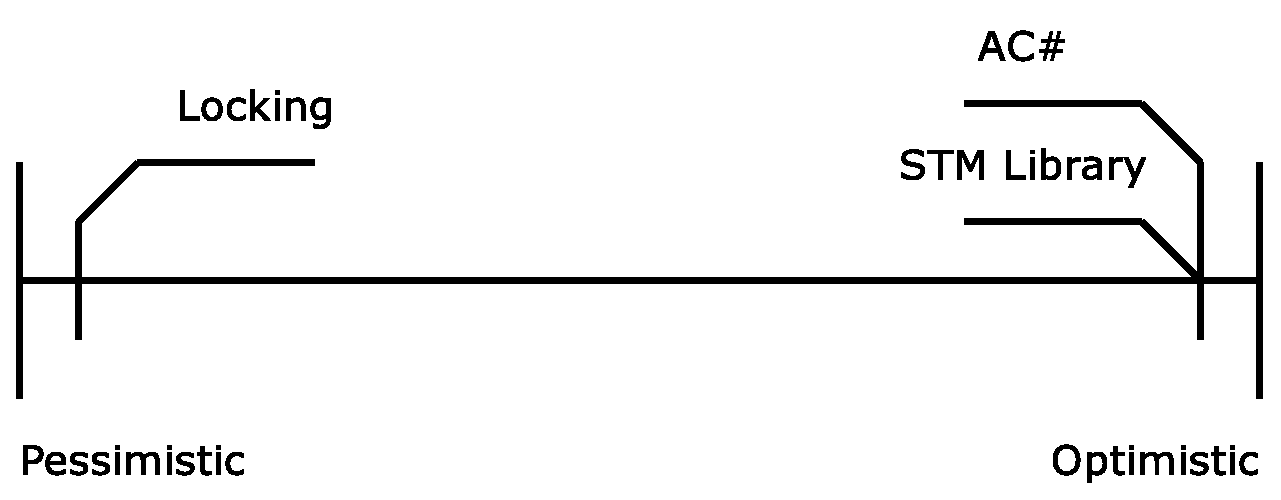
\includegraphics[width=0.9\textwidth]{\rootpath/worksheets/evaluation/figures/char_pessimistic_optemistic} 
 \caption{Concurrency approaches on the pessimistic - optimistic spectrum}
\label{fig:char_pes_opti}
\end{figure}

\subsection{Readability \& Writability}\label{subsec:tl_charac_read_and_write}
As mentioned in \bsref{sec:readability} and \bsref{sec:writablity}, the evaluation of readability and writablity will be based upon the evaluation of the sub characteristics, on which they are based. As two of these, simplicity and orthogonality, are common for both readability and writability, an evaluation of these is presented first. After this, an evaluation of the readability properties of the \ac{TL} concurrency model is presented, followed by the evaluation of \ac{TL} concurrency models level of abstraction and expressivity. Finally an evaluation of the writability of the \ac{TL} concurrency model is presented.
\kasper[inline]{From old report}

%that of simplicity and orthogonality as well as a number of other considerations. Simplicity and orthogonality is described in the following sections followed by a final evaluation of readability.
\subsubsection{Low or High Simplicity}\label{subsec:simplicity}
\begin{figure}[htbp]
\centering
 \includegraphics[width=0.9\textwidth]{\rootpath/worksheets/evaluation/figures/char_read_simplicity} 
 \caption{Concurrency approaches on the low - high simplicity spectrum}
\label{fig:char_simplicity}
\end{figure}

\subsubsection{Low or High Orthogonality}\label{subsec:orthogonality}

\begin{figure}[htbp]
\centering
 \includegraphics[width=0.9\textwidth]{\rootpath/worksheets/evaluation/figures/char_orthogonality} 
 \caption{concurrency approaches on the low - high orthogonality spectrum}
\label{fig:char_orthogonality}
\end{figure}

\subsubsection{Low or High Readability}
\label{subsec:char_readability}

\begin{figure}[htbp]
\centering
 \includegraphics[width=0.9\textwidth]{\rootpath/worksheets/evaluation/figures/char_readability} 
 \caption{Concurrency approaches on the low - high readability spectrum}
\label{fig:char_readability}
\end{figure}

\subsubsection{Low or High Level of Abstraction}\label{subsec:level_of_abstraction}
Locking is tightly coupled with the hardware architecture through hardware instructions such as Test-and-set and Compare-and-swap\cite[p. 1990]{scott2011sync}. Furthermore low-level abstraction threads is used in order to introduce concurrency. Additionally the programmer have to state exactly how synchronization should be applied using locks. Therefore locking is placed close to the low level of abstraction extreme of the spectrum. However the C\# \bscode{lock} statement, which provides a small abstraction over the release of a lock, keeps it from being at the extreme.

The \ac{STM} approaches also rely on threads, but provide a more high level of abstraction approach for synchronization. \ac{STM} uses transactions, where code segments is marked and the details of how synchronization is achieved is abstracted away to the \ac{STM} system. However the isolation level can pose a threat to the level of abstraction of transactions, as under weak isolation the \ac{STM} will not take non-transactional code into account and the programmer must therefore manage it themselves. In the case of \stmnamesp this is not problematic, as it facilities strong atomicity, as described in \bsref{sec:design_strong_weak_atomicity} and the \ac{STM} system will therefore manage both transactional and non-transactional code. Based on the above, the general \ac{STM} approach lies between the middle and high end of the spectrum, where the main negative factors is that the programmer still have to manage threads and mark regions of code that should be synchronized.
As to the actual placements, there are also some differences in the level of abstraction in 

As to the language \ac{STM} and library \ac{STM} individually, there are some differences in the level of abstraction. Library \ac{STM} requires the programmer to use static method calls, wrap transactional code in lambdas, wrap transactional variables in a \bscode{TMVar}, use the \bscode{Value} property when getting or setting a value, supply \bscode{orelse} transactions as arguments to the atomic method call and write return in front of the static method call if the lambda within can return a value. Many of these concerns is abstracted away or handled more gracefully in the language based \ac{STM}.\toby{Evt. refer ned til expressivity, hvor det vil blive vist med et kodeeksempel. Evt. også sig at de kan se kodeeksemplet dernede (Ellers skal jeg sætte det herop og refere dernede til det herop.} Language \ac{STM} is therefore considered to have a higher level of abstraction than library \ac{STM}.

The placement of the three concurrency approaches on the low level of abstraction - high level of abstraction spectrum is depicted in \bsref{fig:char_level_of_abstraction}. 

\toby[i]{Måske tilføj noget med: obstructed by transactions combining poorly with some existing language constructs, such as exceptions and IO, as described in Section 5.2.3 and Section 5.2.4. (for at begrunde ikke så høj placering)}

\begin{figure}[htbp]
\centering
 \includegraphics[width=0.9\textwidth]{\rootpath/worksheets/evaluation/figures/char_level_of_abstraction} 
 \caption{Concurrency approaches on the low - high level of abstraction spectrum}
\label{fig:char_level_of_abstraction}
\end{figure}

\subsubsection{Low or High Expressivity}\label{subsec:expressivity}
\toby[i]{Ikke færdig endnu}

%noget generelt først om expressivity også forklar ud fra eksempel mellem library og lang base

%evt. prøv at tælle tegn i en library og i en langauge based
A code example from the santa claus problem is shown in the library and language in  \bsref{lst:lib_SleepUntilAwoken} \bsref{lst:lang_SleepUntilAwoken}, respectively. The method ensures that santa sleeps until he is awoken by either three elfs at his door, or all reindeers back from vacation ready to fly his sleigh. \bsref{lst:lang_SleepUntilAwoken} shows the atomic keyword abstracting a static call.

\toby[i]{Evt. indsæt eksmpel på brug af en tmvar og noget med brug af value property}

\toby[i]{Evt. refer til appendix hvor kodeeksmeplerne kommer fra præcist}
\begin{lstlisting}[label=lst:lib_SleepUntilAwoken,
  caption={\bscode{SleepUntilAwoken} Method - \ac{STM} Library},
  language=Java,  
  showspaces=false,
  showtabs=false,
  breaklines=true,
  showstringspaces=false,
  breakatwhitespace=true,
  escapechar=~,
  commentstyle=\color{greencomments},
  keywordstyle=\color{bluekeywords},
  stringstyle=\color{redstrings},
  morekeywords={atomic, retry, orelse, var, get, set, ref, out}]  % Start your code-block

  private WakeState SleepUntilAwoken()
  {
    return STMSystem.Atomic(() =>
    {
      if (_rBuffer.Count != SCStats.NR_REINDEER)
      {
        STMSystem.Retry();
      }
      return WakeState.ReindeerBack;
    },
      () =>
      {
        if (_eBuffer.Count != SCStats.MAX_ELFS)
        {
          STMSystem.Retry();
        }
        return WakeState.ElfsIncompetent;
      });
  }
\end{lstlisting}

\begin{lstlisting}[label=lst:lang_SleepUntilAwoken,
  caption={\bscode{SleepUntilAwoken} Method - \ac{STM} Language},
  language=Java,  
  showspaces=false,
  showtabs=false,
  breaklines=true,
  showstringspaces=false,
  breakatwhitespace=true,
  escapechar=~,
  commentstyle=\color{greencomments},
  keywordstyle=\color{bluekeywords},
  stringstyle=\color{redstrings},
  morekeywords={atomic, retry, orelse, var, get, set, ref, out}]  % Start your code-block

  private WakeState SleepUntilAwoken()
  {
    atomic
    {
      if (_rBuffer.Count != SantaClausProblem.NR_REINDEER)
      {
        retry;
      }
      return WakeState.ReindeerBack;
    }
    orelse
    {
      if (_eBuffer.Count != SantaClausProblem.MAX_ELFS)
      {
        retry;
      }
      return WakeState.ElfsIncompetent;
    }
  }
\end{lstlisting}


\begin{figure}[htbp]
\centering
 \includegraphics[width=0.9\textwidth]{\rootpath/worksheets/evaluation/figures/char_expressivity} 
 \caption{Concurrency approaches on the low - high expressivity spectrum}
\label{fig:char_expressivity}
\end{figure}

\subsubsection{Low or High Writability}
\begin{figure}[htbp]
\centering
 \includegraphics[width=0.9\textwidth]{\rootpath/worksheets/evaluation/figures/char_writability} 
 \caption{Concurrency approaches on the low - high writability spectrum}
\label{fig:char_tl_writability}
\end{figure}

\worksheetend
